\documentclass[10pt,a4paper]{article}
\usepackage[utf8]{inputenc} % para poder usar tildes en archivos UTF-8
\usepackage[spanish]{babel} % para que comandos como \today den el resultado en castellano
\usepackage{a4wide} % márgenes un poco más anchos que lo usual
\usepackage{caratula}
\usepackage[noend]{algorithmic} % es para pseudocodigos
\usepackage{hyperref} %links
\usepackage[top=2cm, bottom=2cm, left=2cm, right=2cm]{geometry}
\usepackage{amsmath}
\usepackage{amssymb}
\usepackage[pdftex]{graphicx}
\usepackage{float}
\usepackage{lastpage}

\usepackage{babel}
\usepackage{listings}
\lstset{breaklines=true,numbers=left, stepnumber=1,basicstyle=\footnotesize, xleftmargin=0.7cm}

\usepackage{amsmath}
\usepackage{amsfonts}
\usepackage{amssymb}
\usepackage[utf8]{inputenc}
\usepackage{verbatim}
\usepackage{alltt}
\usepackage{ulem}
\newcommand{\entidad}[2]{\textbf{#1}(#2)}
\newcommand{\primaryKey}[1]{\underline{#1}}
\newcommand{\ForeignKey}[1]{\dashuline{#1}}
\begin{document}

\titulo{Trabajo Pr\'actico I}
\subtitulo{Sistema de Inscripción Mundial de Irlanda 2017}

\fecha{\today}

\materia{Bases de datos}
\integrante{Aldasoro, Agustina}{86/13}{agusaldasoro@gmail.com}
\integrante{Chamo, Nicolás}{282/13}{nicochamo@gmail.com}
\integrante{Previgliano, Fabricio}{430/13}{fjprevi@gmail.com}
\integrante{Zimenspitz, Ezequiel}{155/13}{ezeqzim@gmail.com}

\maketitle
\newpage

\tableofcontents
\newpage

\section{Introducci\'on}

En octubre de 2017 se llevará a cabo el Campeonato Mundial de Taekwon-do ITF en la ciudad de Dublín, Irlanda. Para este evento, los organizadores precisan una aplicación que permita a las escuelas de todo el mundo, inscribir a sus competidores en las diferentes modalidades y categorías.\\

En el siguiente Trabajo se desarrolla el Dise\~no e Implementaci\'on de la Base de Datos que almacena la informaci\'on acorde a los Requerimientos de la ITF.\\

Los puntos clave del problema a resolver son:
\begin{itemize}
\item Las escuelas, quienes presentan a un Maestro Inscriptor, sus Alumnos y los Coachs.
\item Las categor\'ias que est\'an definidas por su modalidad y las distintas clasificaciones pertinentes (G\'enero, Edad y/o Peso).
\item Los \'arbitros, que est\'an clasificados en Jueces, Presidente de Mesa, \'Arbitro Central y Suplentes.
\end{itemize}

En primera instancia presentaremos el modelo entidad relación del problema, junto a sus restricciones. Luego, formalizaremos este modelo pasandolo al Modelo Relacional. Finalmente presentaremos la implementación SQL de estos modelos.
\newpage

\section{Diagrama Entidad Relación}
\subsection{Diagrama}

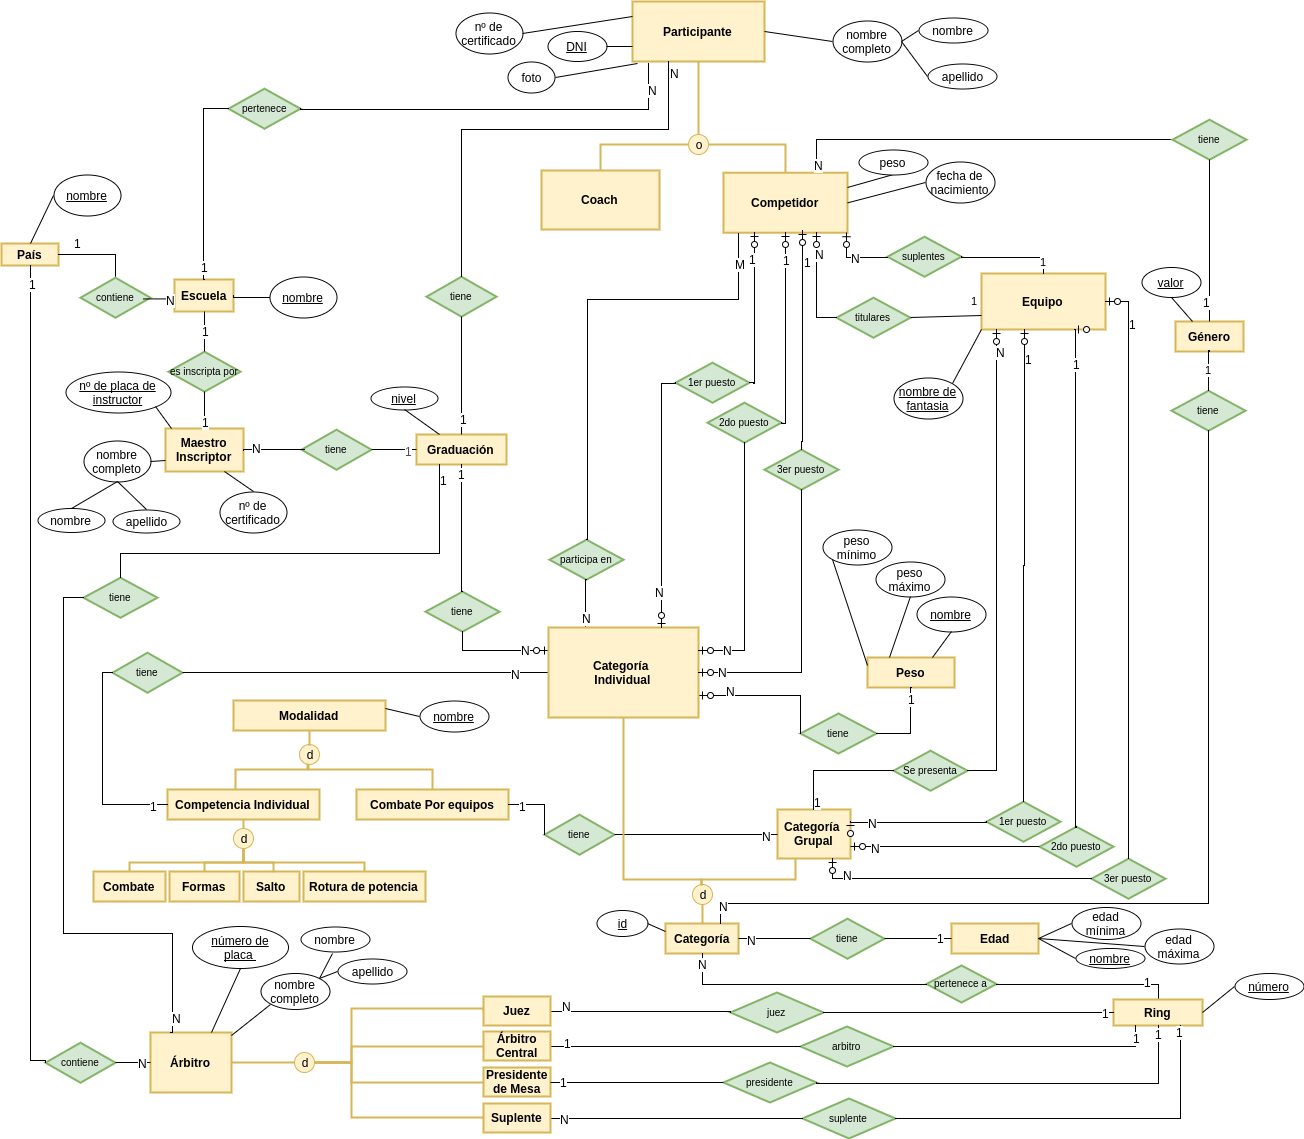
\includegraphics[scale=0.4]{der.png}

\newpage
\subsection{Restricciones}

\begin{enumerate}
\item Por escuela, la cantidad de coachs que presentan es $\lceil$ cantidad de alumnos / 5 $\rceil$.
\item Cada competidor, se puede presentar, a lo sumo, a una categoría de la misma modalidad.
\item Los competidores s\'olo se pueden presentar a categor\'ias que correspondan a sus caracter\'isticas (g\'enero, edad y/o peso).
\item Los equipos están integrados por 5 titulares y 3 suplentes.
\item Cada competidor, si pertenece a un equipo como Titular no debe pertenecer a ning\'un otro como Suplente.
\item Cada competidor, si pertenece a un equipo como Suplente no debe pertenecer a ning\'un otro como Titular.
\item Todos los competidores de un mismo equipo deben pertenecer a la misma escuela.
\item Todos los miembros de un mismo Equipo (titulares y suplentes) deben tener las caracter\'isticas que correspondan a la edad y al g\'enero de la categor\'ia que se presentan.
\item En el ring, los \'arbitros suplentes deben ser al menos 3 y los jueces son m\'as de 1.
\item La graduaci\'on de cada \'arbitro es superior a la graduaci\'on de la categor\'ia que arbitra.
\item El nivel de la graduacion se encuentra entre 1 y 6.
\item Un jugador s\'olo puede pertenecer a la terna de categor\'ias que participa.
\item Dada una categor\'ia individual: si ning\'un competidor se presenta, entonces no puede tener primer, segundo o tercer puesto.
\item Dada una categor\'ia individual: si s\'olo un competidor se presenta, entonces no puede tener segundo o tercer puesto.
\item Dada una categor\'ia individual: si se presentan dos competidores pasa que o bien no tiene ning\'un puesto o tiene primero y segundo.
\item Dada una categor\'ia individual: si se presentan tres competidores o m\'as pasa que o bien no tiene ning\'un puesto o tiene los tres.
\item Dada una categor\'ia individual, los tres primeros puestos son tres personas distintas.
\item Un equipo s\'olo puede pertenecer a la terna de las categor\'ias que participa.
\item Dada una categor\'ia grupal: si ning\'un equipo se presenta, entonces no debe tener primer, segundo o tercer puesto.
\item Dada una categor\'ia grupal: si s\'olo un equipo se presenta, entonces no puede tener segundo o tercer puesto.
\item Dada una categor\'ia grupal: si se presentan dos equipos pasa que o bien no tiene ning\'un puesto o tiene primero y segundo.
\item Dada una categor\'ia grupal: si se presentan tres equipos o m\'as pasa que o bien no tiene ning\'un puesto o tiene los tres.
\item Dada una categor\'ia grupal, los tres primeros puestos son tres equipos distintos.
\item La modalidad ``Combate'' es la \'unica que se clasifica por Peso.
\item La modalidad ``Formas'' es la \'unica que no se clasifica por Graduaci\'on, las dem\'as si.
\item Para todas las categor\'ias que presentan la misma modalidad, si se clasifican por edad, los rangos de edad son disjuntos.
\item Para todas las categor\'ias que presentan la misma modalidad, si se clasifican por peso, los rangos de peso son disjuntos.
\end{enumerate}

\newpage

\section{Modelo Relacional}

\entidad{Maestro Inscriptor}{\primaryKey{n\'umeroDePlacaInstructor}, nombre, apellido, numeroDeCertificado, \ForeignKey{nombreDeGraduación}, \ForeignKey{nombreDeEscuela} }

\textbf{PK} = \textbf{CK} = \{ numeroDePlacaInstructor \}

\textbf{FK} = \{ nombreDeGraduación,nombreDeEscuela \}

\textit{MaestroInscriptor.nombreDeGraduación} debe estar en \textit{Graduación.nombre}

\textit{MaestroInscriptor.nombreDeEscuela} debe estar en \textit{Escuela.Nombre}\\

\entidad{Escuela}{\primaryKey{nombre}}

\textbf{PK} = \textbf{CK} = \{ nombre \}\\

\entidad{País}{\primaryKey{nombre}}

\textbf{PK} = \textbf{CK} = \{ nombre \}\\

\entidad{Graduación}{\primaryKey{nivel}}

\textbf{PK} = \textbf{CK} = \{ nivel \}\\

\entidad{Participante}{\primaryKey{DNI}, n\'umeroDeCertificado, nombre, apellido, \ForeignKey{nombreDeEscuela}, \ForeignKey{nivelDeGraduación}, foto}

\textbf{PK} = \textbf{CK} = \{ DNI \}

\textbf{FK} = \{ nombreDeEscuela, nivelDeGraduación \}

\textit{Participante.nombreDeEscuela} debe estar en \textit{Escuela.nombre}

\textit{Participante.nivelDeGraduación} debe estar en \textit{Graduación.nivel}\\

\entidad{Coach}{\primaryKey{\ForeignKey{DNI}}}

\textbf{PK} = \textbf{CK} = \textbf{FK} = \{ DNI \}

\textit{Coach.DNI} debe estar en \textit{Participante.DNI}\\

\entidad{Competidor}{\primaryKey{\ForeignKey{DNI}}, peso, fechaDeNacimiento, \ForeignKey{suplente}, \ForeignKey{titular}, \ForeignKey{sexo}}

\textbf{PK} = \textbf{CK} = \{ DNI \}

\textbf{FK} = \{ DNI, suplente, titular, sexo \}

\textit{Competidor.sexo} debe estar en \textit{Género.valor}

\textit{Competidor.titular} puede tener o no valor

\textit{Competidor.suplente} puede tener o no valor

\textit{Competidor.titular} debe estar en \textit{Equipo.nombreDeFantasia}

\textit{Competidor.suplente} debe estar en \textit{Equipo.nombreDeFantasia}\\

\entidad{Edad}{\primaryKey{nombre},edadMinima, edadMáxima}

\textbf{PK} = \textbf{CK} = \{ nombre \}\\

\entidad{Peso}{\primaryKey{nombre}, pesoMinimo, pesoMáximo}

\textbf{PK} = \textbf{CK} = \{ nombre \}\\

\entidad{Modalidad}{\primaryKey{nombre}}

\textbf{PK} = \textbf{CK} = \{ nombre \}

\textit{Modalidad.nombre} debe estar en \textit{CompetenciaIndividual.nombre} o (exclusivo) en \textit{CompetenciaIndividual.nombre}\\

\entidad{CompetenciaIndividual}{\primaryKey{\ForeignKey{nombre}}, tipo}

\textbf{PK} = \textbf{CK} = \textbf{FK} = \{ nombre \}

\textit{CompetendiaIndividual.nombre} debe estar en \textit{Modalidad.nombre}\\

\entidad{CombatePorEquipos}{\primaryKey{\ForeignKey{nombre}}}

\textbf{PK} = \textbf{CK} = \textbf{FK} = \{ nombre \}

\textit{CombatePorEquipos.nombre} debe estar en \textit{Modalidad.nombre}\\

\entidad{Equipo}{\primaryKey{nombreDeFantasia}}

\textbf{PK} = \textbf{CK} = \{ nombreDeFantasia \}\\

\entidad{Género}{\primaryKey{valor}}

\textbf{PK} = \textbf{CK} = \{ valor \}

\entidad{Ring}{\primaryKey{numeroDeRing}}

\textbf{PK} = \textbf{CK} = \{ númeroDeRing \}\\

\entidad{Árbitro}{\primaryKey{n\'umeroDePlaca}, nombre, apellido, \ForeignKey{nombreDePaís}, \ForeignKey{graduación}}

\textbf{PK} = \textbf{CK} = \{ numeroDePlaca \}

\textbf{FK} = \{ nombreDePaís, graduación \}

\textit{Árbitro.graduación} debe estar en \textit{graduación.valor}

\textit{Árbitro.nombreDePaís} debe estar en \textit{País.nombre}

\textit{Árbitro.númeroDePlaca} debe estar en \textit{Juez} o en \textit{Árbitro Central} o en \textit{Presidente de Mesa} o en \textit{Suplente}\\

\entidad{Juez}{\primaryKey{\ForeignKey{númeroDePlaca}}, \ForeignKey{númeroDeRing}}
 
\textbf{CK} = \textbf{PK} = \{ númeroDePlaca \}
 
\textbf{FK} = \{ númeroDePlaca, númeroDeRing \}
 
\textit{Juez.númeroDeRing} debe estar en \textit{Ring.númeroDeRing}

\textit{Juez.númeroDePlaca} debe estar en \textit{Ring.númeroDePlaca}\\

\entidad{ÁrbitroCentral}{\primaryKey{\ForeignKey{númeroDePlaca}}, \ForeignKey{númeroDeRing}}

\textbf{CK} = \textbf{PK} = \{ númeroDePlaca \}
 
\textbf{FK} = \{ númeroDePlaca, númeroDeRing \}
 
\textit{ÁrbitroCentral.númeroDeRing} debe estar en \textit{Ring.númeroDeRing}

\textit{ÁrbitroCentral.númeroDePlaca} debe estar en \textit{Ring.númeroDePlaca}\\

\entidad{PresidenteDeMesa}{\primaryKey{\ForeignKey{númeroDePlaca}}, \ForeignKey{númeroDeRing}}

\textbf{CK} = \textbf{PK} = \{ númeroDePlaca \}
 
\textbf{FK} = \{ númeroDePlaca, númeroDeRing \}
 
\textit{PresidenteDeMesa.númeroDeRing} debe estar en \textit{Ring.númeroDeRing}

\textit{PresidenteDeMesa.númeroDePlaca} debe estar en \textit{Ring.númeroDePlaca}

\newpage

\section{Desarrollo}

Detalle de los supuestos asumidos para la resolución del problema.\\

Los jueces no pueden ser suplentes de otro ring y etc.

\newpage

\section{Consultas SQL}

\subsection{Funcionalidades a Implementar}
Código correspondiente a las consultas/stored procedures/ triggers que se piden en el punto Funcionalidades a Implementar.

\lstinputlisting{querysPedidas.sql}

\subsection{Restricciones al Modelo}
Implementación de las restricciones adicionales al modelo utilizando herramientas provistas por la base de datos elegida (triggers, stored procedures, etc).

\lstinputlisting{database.sql}

\newpage

\section{Conclusiones}


\end{document}
